\chapter{\IfLanguageName{dutch}{Datacollectie en Labeling}{Datacollection and Labeling}}%
\label{ch:datacollectie}

\subsection{Doelstelling}
Het doel van deze fase was om een rijke dataset van beeldmateriaal te verzamelen die het gedrag van koeien in een natuurlijke omgeving vastlegt. Deze dataset is gebruikt om de objectdetectiemodellen te trainen die koeien en hun specifieke gedragingen kunnen identificeren en classificeren.


\subsection{Methoden}
\begin{itemize}
  \item \textbf{Data Verzameling:}  Met behulp van een Nvidia Jetson Xavier en een aangesloten camera werd een uitgebreide hoeveelheid videomateriaal verzameld van koeien die zich in een veld bevinden. Deze opzet maakte het mogelijk om real-time videobeelden van hoge kwaliteit vast te leggen die verschillende gedragingen van koeien onder diverse licht- en weersomstandigheden tonen.
  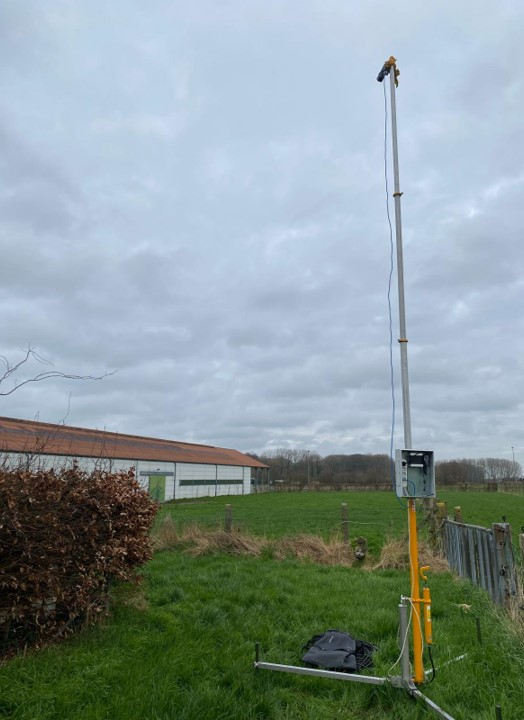
\includegraphics[width=0.5\linewidth]{datacollectie_paal.jpg}
  \item \textbf{Frame Extractie en Voorbereiding:} Het verzamelde videomateriaal werd geconverteerd naar individuele frames om een gedetailleerde analyse en labeling mogelijk te maken. Elk frame vertegenwoordigt een potentiële dataset voor het trainen van de detectiemodellen.
  \item \textbf{Labeling Proces:} De frames werden geüpload naar het platform Labelbox, waar ze manueel gelabeld werden. Voor elk frame werden bounding boxes getekend rond elke koe. Binnen deze boxes werden labels toegevoegd die specifieke gedragingen van de koeien aanduiden, zoals staan, liggen, grazen. Deze stap was cruciaal om nauwkeurige trainingsdata te verstrekken voor het ontwikkelen van effectieve objectdetectie en gedragsclassificatiemodellen.
\end{itemize}

\subsection{Resultaten}
\begin{itemize}
  \item \textbf{Gelabelde Dataset:}  Aan het einde van deze fase werd een uitgebreide dataset verkregen die bestaat uit 3000 gelabelde frames met 5-6 koeien per frame. Deze dataset vormt de basis voor de ontwikkeling en het trainen van de objectdetectie- en gedragsclassificatiemodellen in de volgende fasen van de studie.
  \item \textbf{Datakwaliteit en -variabiliteit:} De kwaliteit en variabiliteit van de data werden verzekerd door de hoge resolutie van de opnamen en de diversiteit in gedrag en omgevingscondities, waardoor de modellen robuust en effectief zullen zijn onder verschillende omstandigheden.
\end{itemize}
\newline
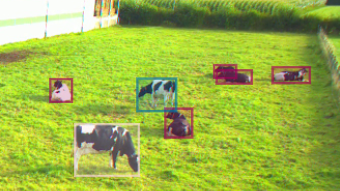
\includegraphics[width=\linewidth]{datacollectie_labeling.png}
\newline